\documentclass[12pt, letterpaper]{article}

\usepackage{algorithm2e}

\usepackage[utf8]{inputenc}
\usepackage{mathtools}
\usepackage[a4paper, total={6in, 9in}]{geometry}
\usepackage{graphicx}

\title{CSE 101 Homework 2}
\author{Kreshiv Chawla, Brian Masse, Taira Sakamoto, Emily Xie}
\date{October 14, 2025}

\begin{document}

\maketitle
\newpage

\begin{enumerate}

%--------------------- Question 1 ---------------------
\item

%--------------------- Question 2 ---------------------
\newpage
\item 
    \textbf{Algorithm.} \newline
    \begin{algorithm}[H]
    $count \gets 0$\;
    \For{each unordered edge $\{u,v\}$ with $A[u][v] = 1$}{
        $S \gets \{ w \in V : A[u][w]=1 \text{ and } A[v][w]=1 \}$\;
        $t \gets 0$\;
        \For{each unordered pair $\{x,y\} \subseteq S$}{
            \If{$A[x][y] = 1$}{
                $t \gets t + 1$\;
            }
        }
        $count \gets count + t$\;
    }
    \Return $count / 6$\;
    \end{algorithm}
    
    \textbf{Correctness.} \medskip \newline
    \textit{Base Case:} If all 6 edges are present, there is exactly 1 4-clique. For each edge ($u,v$), the common neighbor set $S$ has the other 2 vertices. Those two vertices are adjacent, so we add 1 for each of the 6 edges. Total count = 6; dividing by 6 gives 1, which is correct. \medskip \newline
    \textit{Inductive Hypothesis:} Assume the algorithm correctly counts all 4-cliques in any undirected graph with $n=k$ vertices. \medskip \newline
    \textit{Inductive Step:} Consider a graph $G$ with $k+1$ vertices. Let $v_{k+1}$ be the newly added vertex. We can divide 4-cliques in $G$ into two types:
    \begin{enumerate}
        \item 4-cliques not containing $v_{k+1}$: These exist entirely in the subgraph with $k$ vertices. By the inductive hypothesis, the algorithm counts them correctly.
        \item 4-cliques containing $v_{k+1}$: Suppose $v_{k+1}$ is part of some 4-clique $\{v_{k+1},a,b,c\}$. For each edge among these 4 vertices, the intersection $N(a)\cup N(b)$ includes both $v_{k+1}$ and $c$, and since they are connected, the inner loop adds 1. Each 4-clique contributes 6 such additions overall (once per edge). Thus, each new 4-clique is included and counted 6 times. Dividing the final sum by 6 again gives the correct total number of 4-cliques.
    \end{enumerate}
    Therefore, the algorithm correctly counts all 4-cliques in any undirected graph.\medskip
    
    \textbf{Time Complexity.} \medskip \newline
    For each edge $\{u, v\}$, finding $S=N(u)\cup N(v)$ costs $O(|V|)$. Checking all pairs inside $S$ costs $O(|S|^2)$. Summed over all edges, the total time is $O((|V| + |E|)^2)$.

%--------------------- Question 3 ---------------------
\newpage
\item
Let $G$ be a directed graph that is not strongly connected.
We want to make it strongly connected by adding a new vertex $u$ and
as few edges as possible from $u$ to vertices in $G$ and from vertices
in $G$ to $u$.  

\begin{enumerate}

\item Can we ever make $G$ strongly connected by adding $u$ and a single edge
in or out of $u$? Explain your answer.

\-\ \newline
No. Strong Connected requires that \(\forall u \in V\) there is a path to and from \(u\). If we add one edge from \(u\), it becomes a source and there is no way of reaching \(u\). If we add an edge to \(u\), it becomes a sink and there is no way of leaving \(u\). Thus G will not be strongly connected. 
\-\ \newline

\item Give an example of a directed graph with more than one strongly connected component where we can make it strongly connected by adding $u$ and two edges
in or out of $u$?

\[
G: (A, B), (B, C), (C, A), (C, D), (D, E), (E, F)
\]

Add the vertex \(u\) and edges \( (D, u), (u, C) \) to make G strongly connected. 

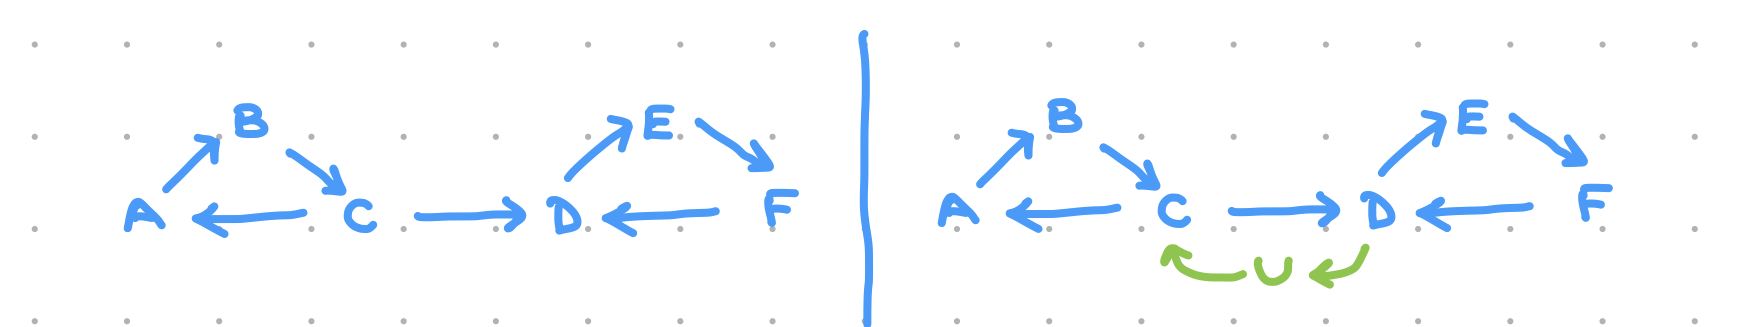
\includegraphics[width=0.9\textwidth]{src/CSE101 hw2 q3.png}


\item Give a characterization (an if and only if condition) of the minimum number of edges we must add,
in terms of the strongly connected components of $G$.

\-\ \newline 
The minimum number of edges \(E_m\) is given by
\[
E_m = S + K
\]

where K is the number of sink SCCs, and S is the number of source SCCs.
\-\ \newline

\item Describe how to use an algorithm from class to compute this number.

\begin {enumerate}
\item Run the Tarjan-Koseraju algorithm to find all SCCs within the graph. 
\item Check whether each SCC is a sink in G by running a DFS algorithm on it. If a node outside the SCC is reachable, it is not a sink. If the only nodes that are reachable are those in the SCC, it is a sink.
\item Repeat items \(i, ii\) for the reverse graph to find its sinks, and thus the regular graph's sources. 

\end {enumerate}

\-\ \newline
\item How long would this algorithm take to do this?  Explain.  

\-\ \newline

The algorithm runs in \(O( |V| (|V| + |E|) )\)

\begin {enumerate}
\item The two Tarjan-Koseraju algorithms run in \(O(|V + |E|)\) time.
\item Each DFS call runs in \(O(|V| + |E|)\), and is run for every vertex at most twice. 
\item Thus the total algorithm takes \(O(|V|(|V| + |E|))\)
\end {enumerate}

\end{enumerate}

%--------------------- Question 4 ---------------------
\newpage
\item

\end{enumerate}
\end{document}

